\documentclass[../main.tex]{subfiles}
\graphicspath{{\subfix{../images/}}}

\begin{document}

\subsection{Κατάτμηση δειγμάτων}

Κατά τη διάρκεια του καρδιακού κύκλου,η καρδιά παράγει ηλεκτρική δραστηριότητα,
η οποία στη συνέχεια προκαλεί κολπικές και κοιλιακές συσπάσεις. Αυτό με την
σειρά του οδηγεί το αίμα γύρω από το σώμα. Το άνοιγμα και το κλείσιμο των
καρδιακών βαλβίδων σχετίζεται με επιταχύνσεις επιβραδύνσεις του αίματος,
προκαλώντας δονήσεις ολόκληρης της καρδιακής δομής. Αυτές οι δονήσεις ακούγονται
στα θωρακικά τοιχώματα και η ακρόαση συγκεκριμένων καρδιακών ήχων μπορεί να
δώσει μια ένδειξη για την υγεία της καρδιάς. Το φωνοκαρδιογράφημα (PCG) είναι η
γραφική αναπαράσταση μιας εγγραφής καρδιακού ήχου. Ένα τυπικό PCG φαίνεται στην
παρακάτω εικόνα:

\begin{figure}[H]
	\center
	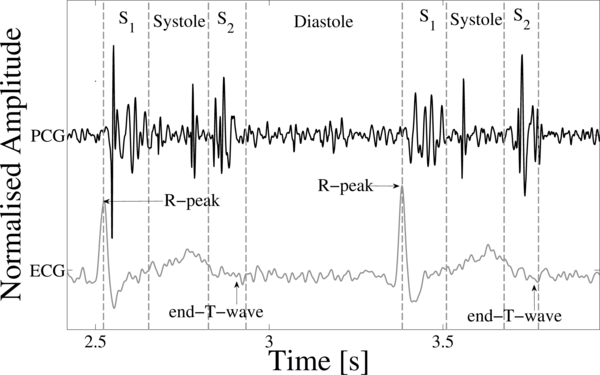
\includegraphics[width=0.7\textwidth]{../images/pcg.png}
	\caption{PCG}
	\label{fig:s1}
\end{figure}


\begin{figure}[H]
	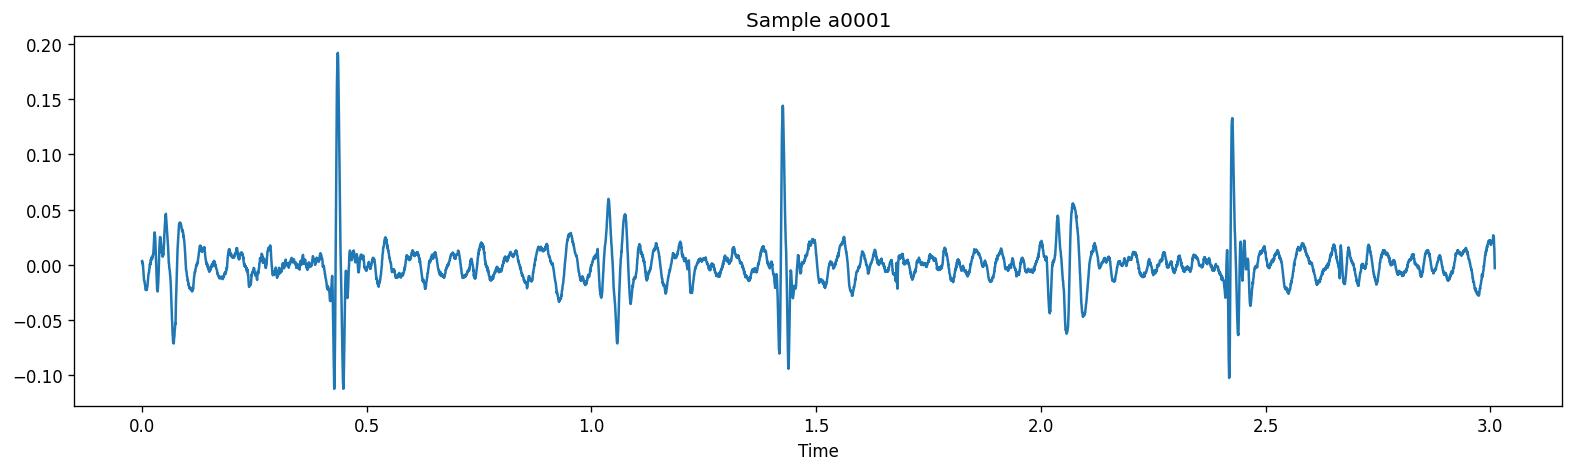
\includegraphics[width=\textwidth]{../images/a0001.png}
	\caption{Αναπαράσταση ήχου με αρχή το πρώτο S1 και διάρκεια 3 δευτερόλεπτα}
	\label{a0001_sound}
\end{figure}

Όπως φαίνεται και στην εικόνα ένας πλήρης καρδιακός κύκλος στο φωνοκαρδιογράφημα
αποτελείται από τέσσερις διακριτές περιοχές. Αυτές είναι οι S1, συστολή, S2 και
διαστολή. Και οι τέσσερις ήχοι που αποτελούν ένα κύκλο σχετίζονται με το
κλείσιμο συγκεκριμένων βαλβίδων και την ροή αίματος από και πρoς τις κοιλίες.

Προκειμένου να διαχωρίσουμε τα PCG που έχουμε στην διάθεσή μας στα παραπάνω
μέρη, χρησιμοποιούμε τον αλγόριθμο του Springer\cite{springer2015logistic}, τον
οποίο  παρείχε ο διαγωνισμός στους συμμετέχοντες. Ο αλγόριθμος αυτός εντοπίζει
τα σημεία εκείνα στα οποία ξεκινάει κάθε ένα από τα στάδια που αναφέρθηκε
παραπάνω (S1, S2, συστολή, διαστολή). Στην συνέχεια, κρατάμε το σημείο στο οποίο
ξεκινάει το πρώτο S1 και κρατάμε 3 δευτερόλεπτα, από αυτό και μετά. Αυτή η
διαδικασία θα γίνεται ώστε τα δείγματα με τα οποία θα εκπαιδεύσουμε το νευρωνικό
δίκτυο να είναι "ευθυγραμμισμένα" μεταξύ τους.

\end{document}
